\RequirePackage{rotating}
%%%%%%%% Document Styles and Packages %%%%%%

\documentclass{amsart}  

\usepackage[foot]{amsaddr}
\usepackage[page]{appendix}

\usepackage[usenames, dvipsnames]{color}
\usepackage{amsfonts}
\usepackage{amsthm}
\usepackage{amsmath}
\usepackage{amsfonts}
\usepackage{latexsym}
\usepackage{amssymb}
\usepackage{amscd}
\usepackage[latin1]{inputenc}
\usepackage{verbatim}
\usepackage{enumerate}
\usepackage{enumitem}
\usepackage{graphicx}
\usepackage{xcolor}
%\usepackage{tkz-berge}
\usepackage{tikz}
\usepackage{tikzpagenodes}
\usepackage{caption}
\usepackage{adjustbox}
%=============================
\usepackage{algorithm2e}
\usepackage{algorithmic}
\usepackage{epstopdf}
\usepackage{fancybox}
\usepackage{booktabs} 
\usepackage{expl3}
\usepackage{l3keys2e}
\usepackage{xparse}
\usepackage{blkarray}
\usepackage{pst-node}
\usepackage{subcaption}
\usepackage{animate}
%\usepackage{tkz-graph}
\usepackage{float}
%\usepackage[table]{xcolor}
%\usepackage{kbordermatrix}
%\usepackage{nicematrix}
\usepackage{booktabs}
\usepackage{makecell}
\usepackage{systeme}
\usepackage{placeins}
\usepackage{young, pst-node}
\usepackage{blindtext}
%=============================
\usetikzlibrary{matrix}
\usetikzlibrary {positioning}
\usetikzlibrary{arrows,shapes}
\usetikzlibrary{trees}
\usetikzlibrary{backgrounds}
\usetikzlibrary{shapes.geometric}
\usetikzlibrary{calc,shapes.callouts,shapes.arrows}
\usetikzlibrary{graphs}
\usetikzlibrary{positioning, arrows}
\usetikzlibrary{fit}

%============================

\definecolor{mybluegreen}{rgb}{0.1, 0.55, 0.35}
\usepackage{caption}
\usepackage{array,booktabs}
\usepackage{rotating}
%%%%%%%%%%%%%%%%%%%%%%%%%%%%%%%%%%%

\usepackage[spaces,hyphens]{url}
\usepackage[colorlinks,allcolors=blue]{hyperref}
\setlength\defaultaddspace{0.5ex}
\usepackage[math]{cellspace}
\setlength\cellspacetoplimit{3pt}
\setlength\cellspacebottomlimit{3pt}

%%%%%%%%%%%  Environments  %%%%%%%%%%%%%%%% 

\newtheorem{theorem}{Theorem}[section]
\newtheorem{lemma}[theorem]{Lemma}
\newtheorem{proposition}[theorem]{Proposition}
\newtheorem{cor}[theorem]{Corollary}
\newtheorem{example}[theorem]{Example}
\newtheorem{conjecture}[theorem]{Conjecture} 
\newtheorem{rem}[theorem]{Remark}
\newtheorem{definition}[theorem]{Definition}
\newtheorem{corollary}[theorem]{Corollary}
\newtheorem{conj}{Conjecture}[section]
% \newtheorem{procedure}{Procedure}[section]
\newtheorem{question}{Question}[section]
\newtheorem{quest}{Question for US}[section]
\theoremstyle{definition}
\DeclareMathOperator{\mr+}{mr_{+}}
\DeclareMathOperator{\M+}{M_{+}}
%\DeclareMathOperator{\mr}{mr}
%\DeclareMathOperator{\M}{M}
\DeclareMathOperator{\nul}{null}
\DeclareMathOperator{\tr}{tr}
\DeclareMathOperator{\one}{\bf 1}
\DeclareMathOperator{\rk}{rank}
%\newtheorem{definition}{Definition}[section]
%\newtheorem{conjecture}{Conjecture}[section]

\newcommand{\Sym}{\mathrm{Sym}} 
\newcommand{\ind}{\mathrm{ind}}
\DeclareMathOperator{\spanof}{span}

\newcommand{\Diff}[1]{D_{#1}}
\newcommand{\diff}[1]{d_{#1}}
\newcommand\fld{{\mathbb F}}
\newcommand\flde{{\mathbb E}}
\newcommand\cS{{\mathcal S}}
\newcommand\cC{{\mathbb{C}}}

\newcommand{\Mod}[1]{\ (\mathrm{mod}\ #1)}
\newcommand\bigzero{\makebox(0,0){\text{\huge0}}}

\newlength{\casewd}
\setlength{\casewd}{\widthof{\bfseries Case 0.}}%
\newlist{caseof}{enumerate}{1}
\setlist[caseof,1]{label = Case \arabic*: , wide=0pt, leftmargin=\dimexpr\casewd + \labelsep, font=\bfseries, topsep=2pt, itemsep=0pt}%

\newlist{subcaseof}{enumerate}{1}
\setlist[subcaseof,1]{
    label = Case (\alph*): ,
    wide = 0pt,
    leftmargin = *,
    font = \bfseries,
    topsep = 2pt,
    itemsep = 0pt
}

%\newcommand\HMD{Weakly Hadamardable}
\definecolor{mybluegreen}{rgb}{0.1, 0.55, 0.35}
%______________________________________________________________
%~~~~~~~~~~~~~~~~~~~~~~~~~~~~~~~~~~~~~~~~~~~~~~~~~~~~~~~~~~~~~~
\title[]{Exploring perfect binary trees with relation to the HK-property}

\author[Atishaya Maharjan]{Atishaya Maharjan} \email[Atishaya Maharjan]{maharjaa@myumanitoba.ca}
\author[M.~N.~Shirazi]{Mahsa N. Shirazi} \email[M.~N.~Shirazi]{mahsa.nasrollahi@gmail.com}
\address{Department of Mathematics, University of Manitoba, Winnipeg,  R3T 2N2,
Canada}


\date{\today}

\keywords{EKR, HK-property, Perfect binary trees, Independence number}
\subjclass[2010]{%05E30, 05C50, 05C25
}

\begin{document}

%______________________________________________________________
%~~~~~~~~~~~~~~~~~~~~~~~~~~~~~~~~~~~~~~~~~~~~~~~~~~~~~~~~~~~~~~
\begin{abstract}
	A perfect binary tree is a full binary tree in which all leaves have the same depth. A set of cocliques of size $k$ ($k$-coclique) in a graph, containing a fixed vertex $v$ is called a star, and is denoted by $\mathcal{I}^n_G(v)$. We study the size of stars for different vertices in a perfect binary tree. This structure is useful in studying the Erd\H{o}s-Ko-Rado theorem. Hurbert and Kumar conjectured that in trees, the largest stars are on the leaves. The conjecture was shown to be false independently by Baber, Borg, and Feghali, Johnson and Thomas. However, in some classes of trees such as caterpillars, the conjecture holds true. In this paper, we study the perfect binary trees through the lens of star centers and seek to answer if the HK-property holds for perfect binary trees. We give an formula and an inductive proof for the independence number of a perfect binary tree and show that the HK-property holds for perfect binary trees. We then show that the proof structure supports any perfect $m$-nary tree, where $m$ is a natrual number. Finally, we use an algorithm by Niskanen and R. J. to generate all cocliques of a perfect binary tree of depth $d$ and compare the number of $k$-cocliques containing a vertex $v$ and a leaf $l$ to see, numerically, if the HK-property holds for perfect binary trees.
\end{abstract}

%______________________________________________________________
%~~~~~~~~~~~~~~~~~~~~~~~~~~~~~~~~~~~~~~~~~~~~~~~~~~~~~~~~~~~~~~
\maketitle

%______________________________________________________________
%~~~~~~~~~~~~~~~~~~~~~~~~~~~~~~~~~~~~~~~~~~~~~~~~~~~~~~~~~~~~~~
\section{Introduction and Preliminaries}
For a given graph $G = (V,E)$, $V(G)$ and $E(G)$ denotes the vertex sets and edge sets of the graph $G$. For an arbitrary vertex, $v \in V(G)$, all vertices adjacent to $v$ are called the neighbours of $v$ and the set of neighbours of $v$ is denoted by $N_G(v)$. The degree of a vertex $v \in V(G)$ is the cardinality of the set of neighbours of $v$, and is denoted by $deg_G(v)$.

For $n \in \mathbb{Z^+}$ such that  $0 \leq n \leq |V(G)|$, a path of length $n$ in $G$ is a sequence of distinct vertices $v_1, v_2, \ldots, v_n$ such that $v_i$ is adjacent to $v_{i+1}$ for $1 \leq i \leq n-1$ and it is called a $uv$-path. A cycle is an extension of a path such that the last vertex is connected to the first vertex, i.e for a path of length $n$, $v_nv_i \in E(G)$. As such, the length of the cycle is $n + 1$.

A connected graph is a graph if for all $u,v \in V(G)$, there exists a $uv$-path. A coclique is a set of vertices such that no two vertices in the set are adjacent to each other. We denote a family of indpendent sets of a graph $G$ by $I_G$. A family of coclique of size $n$ in a graph $G$ is denoted by $\mathcal{I}^n_G$. For $v \in V(G)$, the family of indpendent sets, $\mathcal{I}^n_G(v) := \{A \in \mathcal{I}^n_G : v \in A\}$ is called a star of $\mathcal{I}^n_G$ and $v$ is called its center.

A tree is a connected graph with no cycles, it is denoted by $T$. For a vertex $v \in V(T)$, if $deg_T(v) = 1$, it is called a leaf. A vertex that is not a leaf is called an interior vertex. The vertex at the top which branches $2$ children is called the root vertex and is denoted by $r$. The depth of a vertex is defined as the cardinality of the set of vertices of the path from the root vertex to it. The parent of a vertex $v$ is the vertex connected to $v$ on the path to $r$. A child of a vertex $v$ is a vertex of which $v$ is the parent. We study a more particular class of trees called binary trees, denoted by $T_B$, where each interior vertex $v$ has exactly $2$ children and all leaves have the same depth. Further, a perfect binary tree is a binary tree in which every vertex $v \in V(T)$ has either $0$ or $2$ children. A perfect binary tree is denoted by $T_{PB}$, however in this paper we will simply drop the subscript and denote it as $T$ for clarity. A level $n$ of a perfect binary tree is a set of vertices such that all vertices in the set have a depth of $n$. A perfect $m$-nary tree is a tree in which every vertex $v \in V(T)$ has either $0$ or $m$ children, where $m \in \mathbb{Z}^+$.

The star centers of a graph are interesting because they relate to the EKR theorem.

The Erd\H{o}s-Ko-Rado (EKR) theorem limits the number of sets in a family of sets that can be pairwise intersecting. The theorem states that for a family of $k$-sets of a ground set of size $n$, the maximum number of sets that can be pairwise intersecting is $\binom{n-1}{k-1}$. This theorem has wide applications in combinatorics, graph theory, probability, and other areas of statistics and mathematics.

Studying the EKR theorem, ~\cite{MR2763040} Hulbert and Kamat tried to narrow it down to a more reduced class of graphs called the k-EKR graphs. A graph $G$ is said to be $k$-EKR if for any family of cocliques $\mathcal{F} \subset \mathcal{I}^k_G$ satisfying $A \cap B \neq \emptyset$ for every $A, B \in \mathcal{F}$, there is a vertex $x \in V(G)$ such that $|\mathcal{F}| \leq \mathcal{I}^k_G(v)$. They then conjectured the following:

\begin{conjecture}[k-EKR Conjecture]
	Let $G$ be a graph, and let $\mu(G)$ be the size of its smallest maximal coclique. Then $G$ is $k$-EKR for every $1 \leq k \leq \frac{\mu(G)}{2}$.
\end{conjecture}

\newpage

However, this conjecture is hard to understand and prove, so they narrowed the class of graphs to be trees and gave the following conjecture:

\begin{conjecture}[HK-Property]
	For any $k \geq 1$ and any tree $T$, there exists a leaf $l$ of $T$ such that $|\mathcal{I}^k_T(v)| \leq |\mathcal{I}^k_T(l)|$ for each $v \in V(T)$.
\end{conjecture}

The HK-property holds true for $k \leq 4$, but was proven false independently in ~\cite{MR3271819, MR3612439, MR2523796}. The counterexample that that they arrived at is a type of graph that is defined as a class of trees called $lobster$ ~\cite{MR4245360}.
A tree $C$ is called a $caterpillar$ if $G$ removing the leaves and incident edges produces a path graph $P$, called the spine. A tree $L$ is called a $lobster$ if removing the leaves and incident edges produces a caterpillar $C$.

This is interesting for us as $lobster$ graphs resemble a binary tree.

\begin{figure}[hbt!]
	\centering
	\begin{tikzpicture}[scale=0.7,level distance=2cm,
			level 1/.style={sibling distance=10cm},
			level 2/.style={sibling distance=4cm},
			every node/.style={circle, draw, fill=white, minimum size=1.75em},]
		\node (v11) {$v_0$}
		child {node (v21) {$v_1$}
				child {node  {}
						child {node {}}
					}
				child {node {}
						child {node {}}
					}
				child {node {}
						child {node {}}
					}
			}
		child {node (v22) {$v_2$}
				child {node {}
						child {node {}}
					}
				child {node {}
						child {node {}}
					}
				child {node {}
						child {node {}}
					}
			};
	\end{tikzpicture}
	\caption{The largest k-star for $k \geq 5$ is centered at $v_0$ (A lobster)}
\end{figure}

They figured out that the lobsters, while not completely obeying the HK-property, almost obey the HK-property by either having the largest stars centered around the leaves or at the root of the tree.

\newpage

%~~~~~~~~~~~~~~~~~~~~~~~~~~~~~~~~~~~~~~~~~~~~~~~~~~~~~~~~~~~~~~
\subsection{Some classes of graphs that are HK and a counterexample}

In the paper by Estrugo and Passtine~\cite{MR4245360}, they gave a couple of classes of graphs that have the HK-property. The classes of graphs that they gave were the $caterpillars$ and the $spiders$. The definition of $caterpillars$ is given above. The $spiders$ are trees that only have 1 vertex with degree greater than 2.

\begin{figure}[htb!]
	\begin{subfigure}{0.5\textwidth}
		\centering
		\begin{tikzpicture}[every node/.style={circle, draw, fill=white, minimum size=1.75em}]
			% Draw the path (spine)
			\node (v1) at (0,0) {$v_1$};
			\node (v2) at (2,0) {$v_2$};
			\node (v3) at (4,0) {$v_3$};
			\node (v4) at (6,0) {$v_4$};
			\draw (v1) -- (v2) -- (v3) -- (v4);

			% Draw the leaves
			\node (v7) at (4,2) {$v_7$};
			\node (v8) at (6,2) {$v_8$};
			\node (v9) at (6,-2) {$v_9$};  % New vertex attached to v4
			\draw (v3) -- (v7);
			\draw (v4) -- (v8);
			\draw (v4) -- (v9);  % Edge to the new vertex
		\end{tikzpicture}
		\caption{A caterpillar}
	\end{subfigure}
	\begin{subfigure}{0.5\textwidth}
		\centering
		\begin{tikzpicture}[every node/.style={circle, draw, fill=white, minimum size=1.75em}]
			% Draw the path (spine)
			\node (v1) at (0,0) {$v_1$};
			\node (v2) at (2,0) {$v_2$};
			\node (v3) at (4,0) {$v_3$};
			\node (v4) at (6,0) {$v_4$};
			\draw (v1) -- (v2) -- (v3) -- (v4);

			% Draw the leaves
			\node (v7) at (1,1.33) {$v_7$};
			\node (v8) at (3,1.33) {$v_8$};
			\node (v9) at (1,-1.33) {$v_9$};
			\node (v10) at (3,-1.33) {$v_{10}$};
			\draw (v2) -- (v7);
			\draw (v2) -- (v8);
			\draw (v2) -- (v9);
			\draw (v2) -- (v10);
		\end{tikzpicture}
		\caption{A Spider}
	\end{subfigure}
\end{figure}

%~~~~~~~~~~~~~~~~~~~~~~~~~~~~~~~~~~~~~~~~~~~~~~~~~~~~~~~~~~~~~~
\section{Perfect M-Nary Trees are HK}

\begin{definition}[Maximum Coclique]
	We denote the maximum coclique of a perfect $m$-nary tree of depth $d$ by $\mathcal{I}_d$.
\end{definition}

\begin{conjecture}[HK property for a perfect m-nary tree]
	For any given perfect m-nary tree $T$, the maximum number of cocliques lie in the leaves. The number of cocliques is denoted by $k$. $\alpha(T)$ denotes the independence number of a tree $T$.
\end{conjecture}

%% For perfect m-nary trees
\begin{theorem}\label{theorem:mnary_independence_num}
	For a given perfect $m$-nary tree $T$ with depth $d$ and maximum number of cocliques possible, i.e. $k = \alpha(T)$ we have:
	\begin{align*}
		\alpha(T) = \begin{cases}
			            m^{d - 1} + m^{d-3} + \ldots + 1 \text{ for odd $d$}  \\
			            m^{d - 1} + m^{d-3} + \ldots + m \text{ for even $d$} \\
		            \end{cases}
	\end{align*}

	Or, in summation notation:
	\begin{align*}
		\alpha(T) = \displaystyle\sum_{i = 1}^{\left\lceil \frac{d}{2} \right\rceil} m^{d - 2i + 1}
	\end{align*}
\end{theorem}

\begin{proof}[Proof for ~\ref{theorem:mnary_independence_num}]
	$ $ \\
	We shall proceed by inducting on $d$.\\
	We will have two cases, one for $d$ being odd and another for $d$ being even.
	\begin{caseof}
		\item $d$ is odd \\

		For our base case, consider the trivial case of $d = 1$. Here, $\alpha(T) = 1$. Hence, the base case holds. \\

		Now, say that the statement holds for all $d$. We now have to show that it holds for $d+1$. That is, we need to show that it holds for a given perfect $m$-nary tree $T$ of depth $d + 1$. Note that if $d$ is odd, then $d + 1$ is even. Hence, we expect that:


		\begin{align*}
			\alpha(T) = m^d + m^{d - 2} + \ldots + m
		\end{align*}

		Consider these 2 cases:

		\begin{subcaseof}
			\item $r \in \mathcal{I}_{d + 1}$

			Let $v_i, i \in \{1, \dots, m\}$ be the children of $r$.

			Disregarding the first two depth levels, we obtain that the number of elements in the third depth level is $m^{3-1} = m^2$.

			Let $C_i, i \in \{1,\dots, m^2\}$ be the $m^2$ perfect $m$-nary sub-tree components generated by $T \setminus \{r, v_i\}$.

			If the root $\in \mathcal{I}_{d + 1}$, then $v_i \not\in \mathcal{I}_d$. This means that the remaining vertices of $\mathcal{I}_d$ is in one of the $m^2$ components.
			Since the current depth from the $r$ is $d + 1$, then $T \setminus \{r, v_i\}$ will have depth of $d + 1 - 2 = d - 1$. Since $d$ is odd, then $d + 1$ is even which implies that $d - 1$ is also even.

			By symmetry, it is enough to consider one of the $m^2$ components' maximum coclique for our calculations. Since the $m^2$ components are disjoint, then we can add their independence numbers together along with the $r$ and obtain the following:
			\begin{align*}
				\alpha(T_{d + 1}) = m^2(\alpha(T_{d - 1})) + 1
			\end{align*}

			Then, from our induction hypothesis, we get that:

			\begin{align}
				\alpha(T_{d+1}) & = m^2\underbrace{(m^{d - 2} + m^{d - 4} + \ldots + m)}_{\frac{d-1}{2} \text{terms}} + 1                           \nonumber \\
				                & = m^2\displaystyle\sum_{i = 1}^{\frac{d-1}{2}}m^{d - 2i} + 1
				\label{eq:mnary_odd_case}
			\end{align}


			\item $r \not\in \mathcal{I}_{d + 1}$

			If $r \not\in \mathcal{I}_{d + 1}$, then the remaining elements of $\mathcal{I}_{d + 1}$ are from $T \setminus \{r\}$.

			Let $T' = T\setminus\{r\}$. Then $T'$ is a forest of $m$ disjoint and distinct components. Let $C_i, i \in \{1, \dots, m\}$ be the $m$ components of $T'$. Since $T$ was a perfect $m$-nary tree of depth $d + 1$, then all $C_i$ are also perfect $m$-nary subtrees of depth:
			\begin{align*}
				 & = (d + 1) - 1 \\
				 & = d
			\end{align*}

			Since $d$ is odd, and all $C_i$ are disjoint and distinct perfect $m$-nary subtrees,
			\begin{align*}
				\alpha(T') = \displaystyle\sum_{i = 1}^{m}\alpha(C_i)
			\end{align*}

			By symmetry we get that,
			\begin{align*}
				\alpha(T') = m \alpha(C_1)
			\end{align*}

			Since $r \not\in \mathcal{I}_d$,
			\begin{align*}
				\alpha(T) = \alpha(T') = m \alpha(C_1)
			\end{align*}

			Then, by our induction hypothesis,
			\begin{align}
				\alpha(T) & = m\underbrace{(m^{d - 1} + m^{d - 3} + \dots + 1)}_{\left\lceil\frac{d}{2}\right\rceil \text{terms}}          \nonumber \\
				          & = m\left(\displaystyle\sum_{i = 1}^{\left\lceil\frac{d}{2}\right\rceil}m^{d - (2i - 1)}\right) \nonumber
			\end{align}

			Note that $\left\lceil\frac{d}{2}\right\rceil = \frac{d + 1}{2}$, since $d$ is odd, then,
			\begin{align}
				\alpha(T) & = m\left(\displaystyle\sum_{i = 1}^{\left\lceil\frac{d}{2}\right\rceil}m^{d - (2i - 1)}\right) \nonumber \\
				          & = m\left(\displaystyle\sum_{i = 1}^{\frac{d + 1}{2}}m^{d - (2i - 1)}\right)  \label{eq:mnary_even_case}
			\end{align}


		\end{subcaseof}

		Since $\alpha(T)$ is the maximum coclique,
		\begin{align*}
			\alpha(T) = \max(\ref{eq:mnary_odd_case}, \ref{eq:mnary_even_case})
		\end{align*}

		Remember that our objective is to show that $\alpha(T) = (\ref{eq:mnary_even_case})$ as this aligns with our inductive hypothesis.

		From (\ref{eq:mnary_even_case}), we can simplify it as the following:

		\begin{align*}
			\alpha(T) & = m\left(\displaystyle\sum_{i = 1}^{\frac{d + 1}{2}}m^{d - (2i - 1)}\right)                                             \\
			          & = m\left(m^{d - 2\left(\frac{d + 1}{2}\right) + 1} + \displaystyle\sum_{i = 1}^{\frac{d - 1}{2}}m^{d - (2i - 1)}\right) \\
			          & = m\left(m^{d - d - 1 + 1} + \displaystyle\sum_{i = 1}^{\frac{d - 1}{2}}m^{d - (2i - 1)}\right)                         \\
			          & = m\left(m^0 + \displaystyle\sum_{i = 1}^{\frac{d - 1}{2}}m^{d - (2i - 1)}\right)                                       \\
			          & = m\left(1 + \displaystyle\sum_{i = 1}^{\frac{d - 1}{2}}m^{d - (2i - 1)}\right)                                         \\
			          & = m\left(1 + \displaystyle\sum_{i = 1}^{\frac{d - 1}{2}}m^{d - 2i + 1}\right)                                           \\
			          & = m\left(1 + m\displaystyle\sum_{i = 1}^{\frac{d - 1}{2}}m^{d - 2i)}\right)                                             \\
			          & = m + m^2\displaystyle\sum_{i = 1}^{\frac{d - 1}{2}}m^{d - 2i}                                                          \\
			          & = m^2\displaystyle\sum_{i = 1}^{\frac{d - 1}{2}}m^{d - 2i} + m                                                          \\
			          & > m^2\displaystyle\sum_{i = 1}^{\frac{d - 1}{2}}m^{d - 2i} + 1                                                          \\
			          & = (\ref{eq:mnary_odd_case})
		\end{align*}

		Which implies that,

		\begin{align*}
			\alpha(T) = \max(\ref{eq:mnary_odd_case}, \ref{eq:mnary_even_case}) = (\ref{eq:mnary_even_case})\; \text{as required.}
		\end{align*}

		\item $d$ is even \\

		We will proceed similarly to the odd case.

		For our base case, consider the case of $d = 2$. It is quite easy to see that the maximum coclique will be made up of all the leaves aside from $m$ which resolves the base case.

		Now, say that the statement holds for all $d$. We now have to show that it holds for $d+1$. That is, we need to show that it holds for a given perfect $m$-nary tree $T$ of depth $d + 1$. Note that if $d$ is even, then $d + 1$ is odd. Hence, we expect that:

		\begin{align*}
			\alpha(T) = m^d + m^{d - 2} + \ldots + 1
		\end{align*}

		Consider these 2 cases:

		\begin{subcaseof}
			\item $r \in \mathcal{I}_{d + 1}$

			Let $v_i, i \in \{1, \dots, m\}$ be the children of $r$.

			Disregarding the first two depth levels, we obtain that the number of elements in the third depth level is $m^{3-1} = m^2$.

			Let $C_i, i \in \{1,\dots, m^2\}$ be the $m^2$ perfect $m$-nary sub-tree components generated by $T \setminus \{r, v_i\}$.

			If the root $\in \mathcal{I}_{d + 1}$, then $v_i \not\in \mathcal{I}_d$. This means that the remaining vertices of $\mathcal{I}_d$ is in one of the $m^2$ components.

			Since the current depth from the $r$ is $d + 1$, then $T \setminus \{r, v_i\}$ will have depth of $d + 1 - 2 = d - 1$. Since $d$ is even, then $d + 1$ is odd which implies that $d - 1$ is also odd.

			By symmetry, it is enough to consider one of the $m^2$ components' maximum coclique for our calculations. Since the $m^2$ components are disjoint, then we can add their independence number together along with the $1$ from $r$ and obtain the following:

			\begin{align*}
				\alpha(T_{d + 1}) = m^2(\alpha(T_{d - 1})) + 1
			\end{align*}

			Since $d - 1$ is odd, from our induction hypothesis, we have that:

			\begin{align*}
				\alpha(T_{d - 1}) = \underbrace{m^{d - 2} + m^{d - 4} + \dots + 1}_{\left\lceil\frac{d - 1}{2}\right\rceil = \frac{d - 1 + 1}{2} = \frac{d}{2} \text{terms}}
			\end{align*}

			Thus, we obtain that $\alpha(T_{d+1})$ becomes the following:

			\begin{align}
				\alpha(T_{d + 1}) & = m^2(\underbrace{m^{d - 2} + m^{d - 4} + \dots + 1}_{\frac{d}{2} \text{terms}}) + 1 \nonumber \\
				                  & = m^2 \displaystyle\sum_{i = 1}^{\frac{d}{2}}m^{d - 2i} + 1
				\label{eq:mnary_even_case_root_in}
			\end{align}

			\item  $r \not\in \mathcal{I}_{d+1}$
			If $r \not\in \mathcal{I}_{d + 1}$, then the remaining elements of $\mathcal{I}_{d + 1}$ are from $T \setminus \{r\}$.


			Let $T' = T\setminus\{r\}$. Then $T'$ is a forest of $m$ disjoint and distinct components. Let $C_i, i \in \{1, \dots, m\}$ be the $m$ components of $T'$. Since $T$ was a perfect $m$-nary tree of depth $d + 1$, then all $C_i$ are also perfect $m$-nary subtrees of depth:
			\begin{align*}
				 & = (d + 1) - 1 \\
				 & = d
			\end{align*}

			Since all $C_i$ are disjoint and distinct perfect $m$-nary subtrees,
			\begin{align*}
				\alpha(T') = \displaystyle\sum_{i = 1}^{m}\alpha(C_i)
			\end{align*}

			By symmetry we get that,
			\begin{align*}
				\alpha(T') = m \alpha(C_1)
			\end{align*}

			Since $r \not\in \mathcal{I}_d$,
			\begin{align*}
				\alpha(T) = \alpha(T') = m \alpha(C_1)
			\end{align*}

			Since $d$ is even and by our induction hypothesis,
			\begin{align}
				\alpha(T) & = m\underbrace{(m^{d - 1} + m^{d - 3} + \dots + m)}_{\frac{d}{2} \text{terms}}           \nonumber \\
				          & = m\left(\displaystyle\sum_{i = 1}^{\frac{d}{2}}m^{d - (2i - 1)}\right)
				\label{eq:mnary_even_case_root_not_in}
			\end{align}

			From (\ref{eq:mnary_even_case_root_not_in}), we see that,

			\begin{align*}
				 & = m\left(\displaystyle\sum_{i = 1}^{\frac{d}{2}}m^{d - (2i - 1)}\right) \\
				 & = m\left(\displaystyle\sum_{i = 1}^{\frac{d}{2}}m^{d - 2i + 1}\right)   \\
				 & = m^2\left(\displaystyle\sum_{i = 1}^{\frac{d}{2}}m^{d - 2i}\right)     \\
				 & < m^2\left(\displaystyle\sum_{i = 1}^{\frac{d}{2}}m^{d - 2i}\right) + 1 \\
				 & = (\ref{eq:mnary_even_case_root_in})
			\end{align*}

			Since $\alpha(T)$ is the maximum coclique,
			\begin{align*}
				\alpha(T) = \max(\ref{eq:mnary_even_case_root_in}, \ref{eq:mnary_even_case_root_not_in}) = (\ref{eq:mnary_even_case_root_in})\; \text{as required.}
			\end{align*}
		\end{subcaseof}
	\end{caseof}

	Thus, by the mathematical induction, our formula for the independence number of a perfect $m$-nary tree holds.
\end{proof}

\begin{corollary}\label{cor:root_in_not_in}
	By $Theorem$ (\ref{theorem:mnary_independence_num}), we see that for perfect $m$-nary trees with odd depth $d$, $r \in \mathcal{I}_d$. For even depth $d$, $r \not\in \mathcal{I}_d$.
\end{corollary}

\begin{theorem}\label{theorem:unique_independence_num}
	Following from the previous Theorem ~\ref{theorem:mnary_independence_num}, we claim that $\mathcal{I}_d$ is unique.
\end{theorem}
\begin{proof}[Proof for ~\ref{theorem:unique_independence_num}]
	$ $ \\

	Let $T$ be a perfect $m$-nary tree of depth $d$. We shall induct on $d$ to show that $\mathcal{I}_d$ is unique.

	For our base case, consider the trivial case of $d = 1$. Then, we see that $\mathcal{I}_d = \{r\}$. In addition, for $d = 2$, it is quite easy to see that $\mathcal{I}_d = \{l_1,\dots, l_m\}$, where $l_i, i \in \{1,\dots, m\}$ are the leaves.

	Now, say that our statement holds for all $d$. We now have to show that it holds for $d + 1$. That is, we need to show that it holds for a given perfect $m$-nary tree $T'$ of depth $d + 1$.

	We shall proceed by cases.

	\begin{caseof}
		\item $d + 1$ is odd \\
		From ~\ref{cor:root_in_not_in}, we know that if $d + 1$ is odd, then $r \in \mathcal{I}_{d + 1}$.
		\\
		If $r \in \mathcal{I}_{d + 1}$, then that means that all the children of $r$ cannot be included in $\mathcal{I}_{d + 1}$. Then the only remaining options are from the subtrees of depth $d - 1$ rooted at the children of the children of $r$.
		\\
		It is important to note that our subtrees are distinct and disjoint components, hence we will not have any overlapping vertices between them. This also means that by symmetry, we can just consider one of the subtrees.
		\\
		Since $d + 1$ is odd, then $d - 1$ is also odd. Hence, we can use our inductive hypothesis to conclude that all the elements for $\mathcal{I}_{d + 1}$ will be made up of distinct disjoint components which implies that $\mathcal{I}_{d + 1}$ is unique.
		\\
		This concludes this case.

		\item $d + 1$ is even \\
		From ~\ref{cor:root_in_not_in}, we know that if $d + 1$ is even, then $r \not\in \mathcal{I}_{d + 1}$.
		\\
		If $r \not\in \mathcal{I}_{d + 1}$, then that means that the remaining vertices of $\mathcal{I}_{d+1}$ are going to be from the subtrees of depth $d$ rooted at the $m$ children of $r$.
		\\
		It is important to note that our subtrees are distinct and disjoint components, hence we will not have any overlapping vertices between them. This also means that by symmetry, we can just consider one of the subtrees.
		\\
		It is important to note that our subtrees are distinct and disjoint components, hence we will not have any overlapping vertices between them. This also means that by symmetry, we can just consider one of the subtrees.
		\\
		Since $d + 1$ is even, then $d$ is odd. Then, we can use case 1 along with our inductive hypothesis to conclude that all the elements for $\mathcal{I}_{d + 1}$ will be made up of distinct disjoint components which implies that $\mathcal{I}_{d+1}$ is unique.
		\\
		This concludes the case.
	\end{caseof}

	Hence, by strong mathematical induction, we see that $\mathcal{I}_{d}$ is unqiue, as required.
\end{proof}

\begin{theorem}[Perfect m-nary trees are HK]\label{theorem:mnary_hk}
	Let $T$ be a perfect $m$-nary tree with depth $d$. Then, $T$ is HK.
\end{theorem}

\begin{proof}[Proof for ~\ref{theorem:mnary_hk}]
	$ $ \\

	Let $T$ be a perfect $m$-nary tree of depth $d$.
\end{proof}


\begin{definition}[Depth Vertex Set]
	Let $T = (V, E)$ be a perfect binary tree of depth $d$. A depth vertex set is the set of all vertices at the same depth. A depth vertex set of depth $i$ is denoted by $\mathcal{D}_i$, for $i \leq d$.
\end{definition}

\begin{definition}[Parent vertex]
	Let $T = (V, E)$ be a perfect binary tree of depth $d$. Let $v \in V$, the vertex adjacent to $v$ having one less depth is called the parent vertex. If $v \in \mathcal{D_i}$, then the parent of $v$ will be included in $\mathcal{D_{i - 1}}$.
\end{definition}

\begin{definition}[Grandparent vertex]
	A grandparent vertex is the parent of the parent vertex of a given vertex $v$.
\end{definition}

\begin{theorem}[Stars around the leaves dominates stars around the root]\label{theorem:leaves_dom_root}
	For a given perfect binary tree $T = (V, E)$	of depth $d$, there exists a leaf $l$ such that $|\mathcal{I}^k_T(l)| > |\mathcal{I}^k_T(r)|.$
\end{theorem}

\begin{proof}[Proof for ~\ref{theorem:leaves_dom_root}]
	$ $ \\

	Due to the symmetric nature of $T$ it is easy to see that $\mathcal{I}^k_T(l)$ is the same for all choices of leaves $l$. We will pick the first leaf from the left, $l$. We will then show that $|\mathcal{I}^k_T(l)| > |\mathcal{I}^k_T(r)|.$

	Firstly, we will count the total number of cocliques of size $k$ that are centered around $r$. We will use an enumerative approach to select $t_i$ vertices from the depth vertex set of depth $i$, $\mathcal{D}_i$, for $i \leq d$. In essence, we will select for all possible depth vertex sets that are not affected by our choice of vertex $t_i$ vertices such that the sum of them will be equal to $k - 1$. Succintly, we want to choose $t_i$ such that:
	\begin{align*}
		\displaystyle\sum_{i = 3}^{d}t_i = k - 1
	\end{align*}

	Since we are counting the star centered at the root $r$, $r$'s children of $\mathcal{D}_2$ cannot be included and hence, our enumeration starts from selecting $t_3$ vertices from $\mathcal{D}_3$.

	There are $\binom{2^{3 - 1}}{t_3} = \binom{2^2}{t_3}$ possible combinations of vertices that you can choose from $\mathcal{D}_3$. Since $T$ is a perfect binary tree, whenever we select a vertex and add it to our coclique, all of it's children in the next depth vertex set invalid selections for that particular coclique. Hence, since we selected $t_3$ vertices from $\mathcal{D}_3$, we cannot select the children of those $t_3$ vertices from $\mathcal{D}_4$. Hence, there are $\binom{2^{4 - 1} - 2t_3}{t_4} = \binom{2^3 - 2t_3}{t_4}$ possible combinations of vertices that you can choose from $\mathcal{D}_4$. A similar pattern continues until you reach the last depth $d$. Overall, the total number of cocliques of size $k$ that include the root $r$ is the following:

	\begin{align}
		|\mathcal{I}^k_T(r)| & = \binom{2^2}{t_3} \binom{2^3 - 2t_3}{t_4} \binom{2^4 - 2t_4}{t_5}\dots \binom{2^{d - 1} - 2t_{d - 1}}{t_d}
		\nonumber
		\\
		                     & = \binom{2^2}{t_3}\displaystyle\prod_{i = 4}^{d} \binom{2^{i - 1} - 2t_{i - 1}}{t_i}
		\label{eq:root_star_card}
	\end{align}

	Now, we calculate the total number of cocliques of size $k$ that are centered around $l$. We will use a similar enumerative method; however we will need to split this counting into cases:

	\begin{caseof}
		\item $r \in \mathcal{I}^k_T(l)$

		We want to choose $t_i$ such that:
		\begin{align*}
			\displaystyle\sum_{i = 3}^{d}t_i = k - 2
		\end{align*}

		Note that we only need to choose the rest of $k - 2$ vertices because $r, l \in \mathcal{I}^k_T(l)$.

		Note that this enumeration differs with our previous enumeration argument due to the fact that the grandparent of $l$ may or may not be included in the counting which will lead to differing number of possible vertices to be selected in a given coclique.

		We can proceed similarly to our calculation of the number of cocliques of size $k$ centered around $r$ with the two following sub cases:

		\begin{subcaseof}
			\item Grandparent vertex of $l$ is selected in $t_{d - 2}$\\
			If the grandparent vertex of $l$ is selected in $t_{d - 2}$, then this case is the same as the one for the enumeration of cocliques containing $r$:
			\begin{align*}
				\binom{2^{d - 1 - 1} - 2t_{d - 1 - 1}}{t_{d - 1}} = \binom{2^{d - 2} - 2t_{d - 2}}{t_{d - 1}}
			\end{align*}
			\item Grandparent vertex of $l$ is not selected in $t_{d - 2}$ \\
			If the grandparent vertex of $l$ is not selected in $t_{d - 2}$, then we have to account for one less vertex that can be selected from $\mathcal{D}_{d - 1}$:
			\begin{align*}
				\binom{2^{d - 1 - 1} - 2t_{d - 1 - 1} - 1}{t_{d - 1}} = \binom{2^{d - 2} - 2t_{d - 2} - 1}{t_{d - 1}}
			\end{align*}
		\end{subcaseof}

		Finally, we also note that since we already included $l$ in our enumeration, we have one less vertex that we can select from for $t_d$:
		\begin{align*}
			\binom{2^{d - 1} - 2t_{d - 1} - 1}{t_d}
		\end{align*}

		Note that our sub cases are independent events and hence we have to add them instead of multiplying them.

		In total, we obtain the number of cocliques of size $k$ centered around $l$ which include $r$ as:

		\begin{align}
			\binom{2^2}{t_3}\binom{2^{d - 1} - 2t_{d - 1} - 1}{t_d}\left(\binom{2^{d - 2} - 2t_{d - 2}}{t_{d - 1}} + \binom{2^{d - 2} - 2t_{d - 2} - 1}{t_{d - 1}}\right)\displaystyle\prod_{i = 4}^{d - 2}\binom{2^{i - 1} - 2t_{i - 1}}{t_i}\label{eq:leaf_star_card_1}
		\end{align}

		This concludes the first case.

		\item $r \not\in \mathcal{I}^k_T(l)$

		We want to choose $t_i$ such that:
		\begin{align*}
			\displaystyle\sum_{i = 2}^{d}t_i = k - 1
		\end{align*}

		Note that we only need to choose the rest of the $k - 1$ vertices because $l \in \mathcal{I}^k_T(l)$. We can proceed similarly to the previous case and differentiate the cases where the grandparent vertex of $l$ is included in $t_{d - 2}$ or not.

		\begin{subcaseof}
			\item Grandparent vertex of $l$ is selected in $t_{d - 2}$\\
			Similarly to the previous case, we get the following expression:
			\begin{align*}
				\binom{2^{d - 2} - 2t_{d - 2}}{t_{d - 1}}
			\end{align*}


			\item Grandparent vertex of $l$ is not selected in $t_{d - 2}$\\
			Similary to the previous case, we also get the following expression:

			\begin{align*}
				\binom{2^{d - 2} - 2_{d - 2} - 1}{t_{d - 1}}
			\end{align*}

		\end{subcaseof}

		Again, we also note that we already included $l$ in our enumeration and thus have one less vertex that we can select from for $t_d$:

		\begin{align*}
			\binom{2^{d - 1} - 2t_{d - 1} - 1}{t_d}
		\end{align*}

		All in all, for this case we obtain the number of cocliques of size $k$ centered around $l$ that do not include $r$ as:

		\begin{align}
			\binom{2^{d - 1} - 2t_{d - 1} - 1}{t_d}\left(\binom{2^{d - 2} - 2t_{d - 2}}{t_{d - 1}} + \binom{2^{d - 2} - 2t_{d - 2} - 1}{t_{d - 1}}\right)\displaystyle\prod_{i = 2}^{d - 2}\binom{2^{i - 1} - 2t_{i - 1}}{t_i}\label{eq:leaf_star_card_2}
		\end{align}

		This concludes the second case.
	\end{caseof}


	We now show that (\ref{eq:leaf_star_card_1}) + (\ref{eq:leaf_star_card_2}) is greater than (\ref{eq:root_star_card}):
\end{proof}

\newpage
%~~~~~~~~~~~~~~~~~~~~~~~~~~~~~~~~~~~~~~~~~~~~~~~~~~~~~~~~~~~~~~
\begin{appendix}
	\section{cocliques Algorithm and Analysis}\label{coclique-algorithm}
	$ $
	To validate our conjecture, we present a simple algorithm to generate all cocliques of a perfect binary tree of cardinality $k$. We then compare the number of cocliques containing a vertex $v$ and a leaf $l$ to see if the HK-property holds for perfect binary trees.

	To begin with, we present the following algorithm to generate a perfect binary tree of depth $n$:

	\RestyleAlgo{ruled}

	\SetKwComment{Comment}{/* }{ */}

	\begin{algorithm}[hbt!]
		\caption{Perfect Binary Tree Generator}\label{alg:tree-generator}
		\KwData{$n \geq 0$, where $n$ is the depth of the perfect binary tree}
		\KwResult{A perfect binary tree graph and its leaves}

		\SetKwFunction{FMain}{perfect\_binary\_tree\_generator}
		\SetKwFunction{FSub}{get\_leaves}

		\SetKwProg{Fn}{Function}{:}{}
		\Fn{\FMain{$n$}}{
			\eIf{$n = 0$}{
				\Return{Graph()}
			}{
				$g \gets Graph()$\;
				$g$.add\_vertices([$2^n$])\;
				\For{$i$ in range($2^n - 1$)}{
					$g$.add\_edge($i$, $2*i + 1$)\;
					$g$.add\_edge($i$, $2*i + 2$)\;
				}
				\Return{$g$}
			}
		}
	\end{algorithm}

	The algorithm will generate a perfect binary tree of this form:
	\begin{figure}[hbt!]
		\centering

		\begin{tikzpicture}[scale=0.7,level distance=2cm,
				level 1/.style={sibling distance=8cm},
				level 2/.style={sibling distance=4cm},
				level 3/.style={sibling distance=2cm},
				every node/.style={circle, draw, fill=white}]
			\node (0) {$0$}
			child {node (1) {$1$}
					child {node (3) {$3$}
							child {node {$\vdots$}}
							child {node {$\vdots$}}
						}
					child {node (4) {$4$}
							child {node {$\vdots$}}
							child {node {$\vdots$}}
						}
				}
			child {node (2) {$2$}
					child {node (5) {$5$}
							child {node {$\vdots$}}
							child {node {$\vdots$}}
						}
					child {node (6) {$6$}
							child {node {$\vdots$}}
							child {node {$\vdots$}}
						}
				};
		\end{tikzpicture}
	\end{figure}

	It is easy to see that the leaves will start with the value of $\left\lfloor\dfrac{2^{n + 1} - 1}{2}\right\rfloor$, where $n$ is the depth of the perfect binary tree.

	\newpage
	So to generate all the leaves of the perfect binary tree of depth $n$, we present the following algorithm:

	\begin{algorithm}[hbt!]
		\caption{Perfect Binary Tree Leaves Generator}\label{alg:leaves-generator}
		\KwData{$n \geq 0$, where $n$ is the depth of the perfect binary tree}
		\KwResult{A perfect binary tree graph's leaves}

		\SetKwFunction{FMain}{perfect\_binary\_tree\_generator}

		\SetKwProg{Fn}{Function}{:}{}
		\Fn{\FMain{$n$}}{
			$num\_vertices \gets 2^{n + 1} - 1$\;
			$leaves \gets []$\;
			$last\_row\_start \gets floor(num\_vertices / 2)$\;
			\For{$vertex$ in range($last\_row\_start$, $num\_vertices$)}{
				$leaves$.append($vertex$)\;
			}
			\Return{$leaves$}
		}
	\end{algorithm}

	We then use the algorithm from ~\cite{Niskanen2003CliquerUG} to generate a coclique of maximum cardinality for our perfect binary tree.

	\begin{algorithm}[hbt!]
		\caption{Maximum Indpendent Set Algorithm}\label{alg:max-independent-set}
		\KwData{A perfect binary tree graph $T$}
		\KwResult{A maximum coclique of $T$}

		\SetKwFunction{FMain}{maximum\_independent\_set}

		\SetKwProg{Fn}{Function}{:}{}
		\Fn{\FMain{$T$}}{
			$cliquer \gets Cliquer(T)$\;
			\Return{$cliquer$.get\_maximum\_independent\_set()}
		}
	\end{algorithm}


	The next couple of pages show the results of the algorithm for a perfect binary tree of depth 4, 5, and 6. The X-axis denotes the vertice's labels (not the actual numbers) and the Y-axis denotes the cardinality of the stars centered around the vertices.

	\begin{figure}[hbt!]
		\caption*{Depth 4}
		\begin{subfigure}[b]{.45\textwidth}
			\centering
			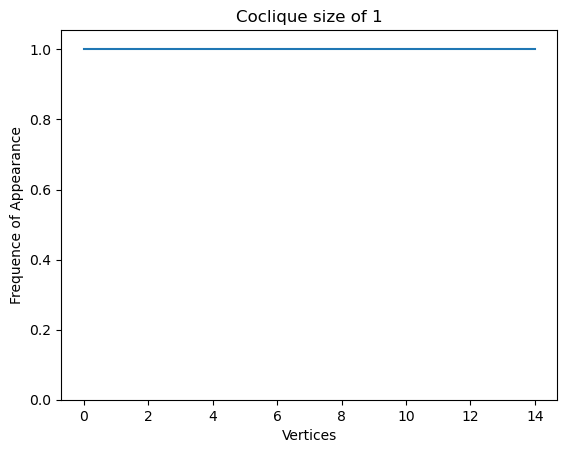
\includegraphics[width=1\linewidth]{depth_4_size_1.png}
			\caption{coclique of size 1}
		\end{subfigure}
		\begin{subfigure}[b]{.45\textwidth}
			\centering
			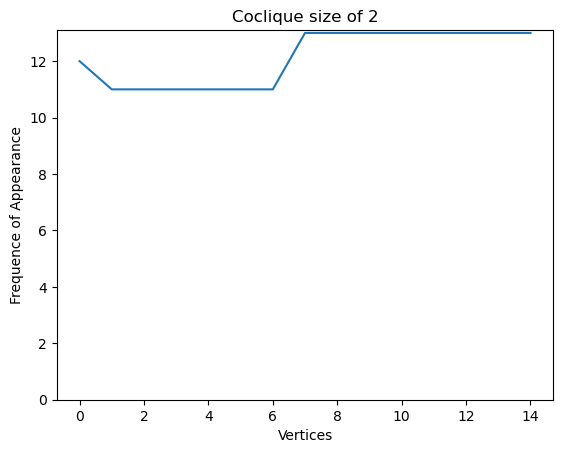
\includegraphics[width=1\linewidth]{depth_4_size_2.png}
			\caption{coclique of size 2}
		\end{subfigure}
		\begin{subfigure}[b]{.45\textwidth}
			\centering
			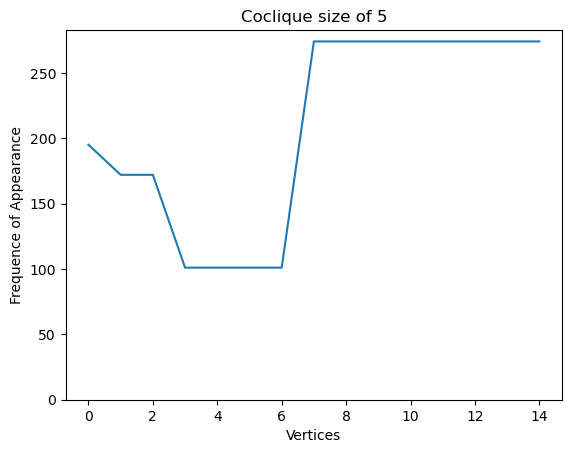
\includegraphics[width=1\linewidth]{depth_4_size_5.png}
			\caption{coclique of size 5}
		\end{subfigure}
		\begin{subfigure}[b]{.45\textwidth}
			\centering
			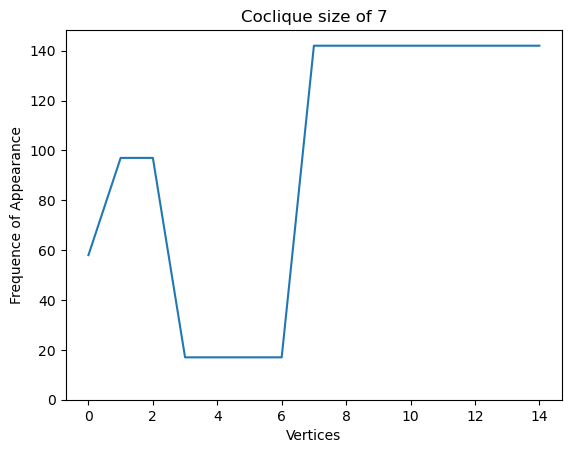
\includegraphics[width=1\linewidth]{depth_4_size_7.png}
			\caption{coclique of size 7}
		\end{subfigure}
		\begin{subfigure}[b]{.45\textwidth}
			\centering
			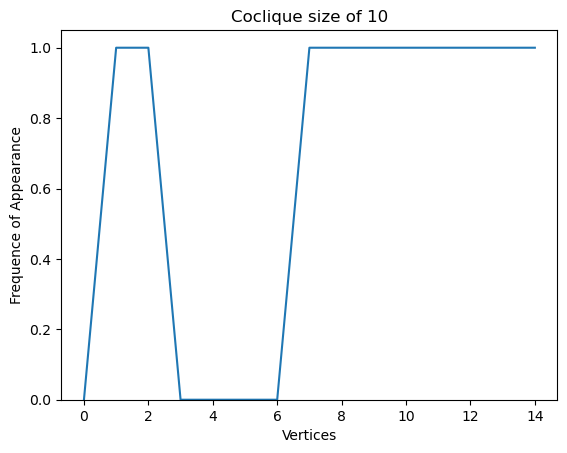
\includegraphics[width=1\linewidth]{depth_4_size_10.png}
			\caption{coclique of size 10}
		\end{subfigure}
	\end{figure}

	\begin{figure}[hbt!]
		\caption*{Depth 5}
		\begin{subfigure}[b]{.45\textwidth}
			\centering
			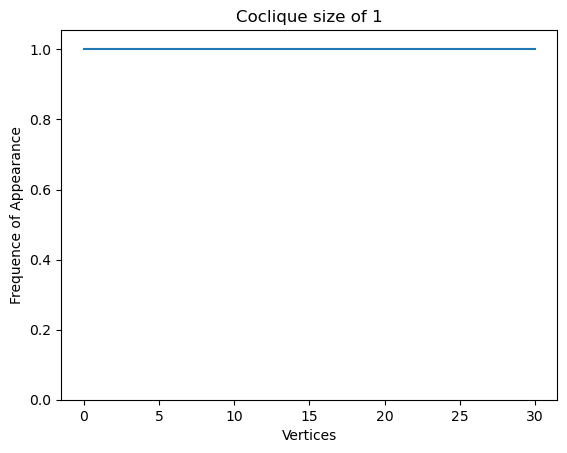
\includegraphics[width=1\linewidth]{depth_5_size_1.png}
			\caption{coclique of size 1}
		\end{subfigure}
		\begin{subfigure}[b]{.45\textwidth}
			\centering
			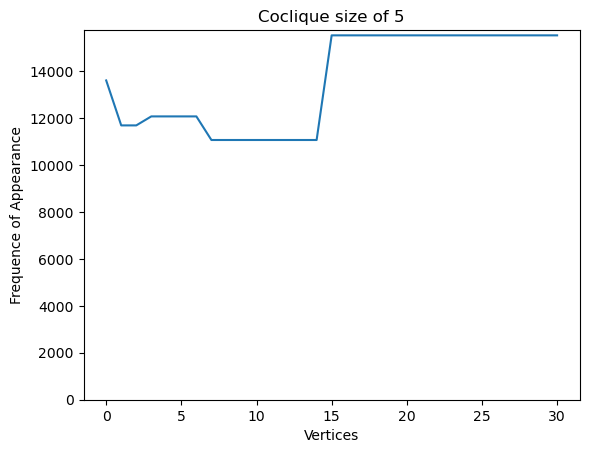
\includegraphics[width=1\linewidth]{depth_5_size_5.png}
			\caption{coclique of size 5}
		\end{subfigure}
		\begin{subfigure}[b]{.45\textwidth}
			\centering
			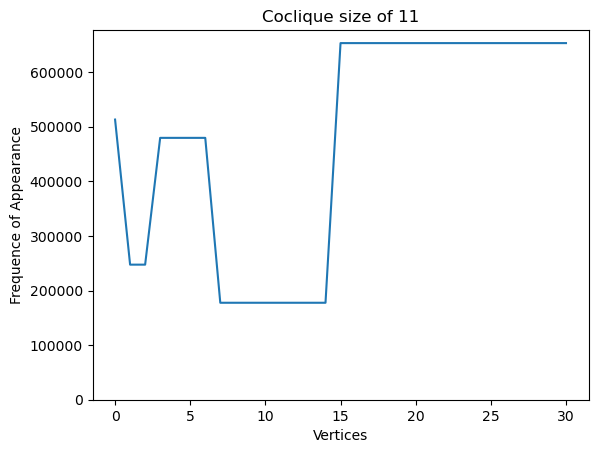
\includegraphics[width=1\linewidth]{depth_5_size_11.png}
			\caption{coclique of size 11}
		\end{subfigure}
		\begin{subfigure}[b]{.45\textwidth}
			\centering
			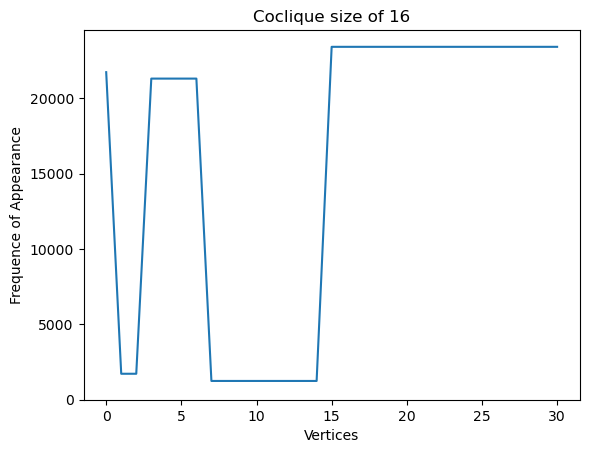
\includegraphics[width=1\linewidth]{depth_5_size_16.png}
			\caption{coclique of size 16}
		\end{subfigure}
		\begin{subfigure}[b]{.45\textwidth}
			\centering
			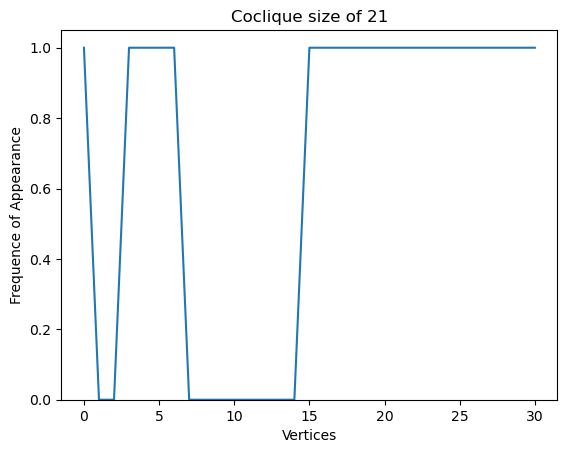
\includegraphics[width=1\linewidth]{depth_5_size_21.png}
			\caption{coclique of size 21}
		\end{subfigure}
	\end{figure}

	The data shown in the figures above verifies that the Partial HK-Property holds for perfect binary trees of depth 5. The next step would be to verify this for perfect binary trees of depth 6 and 7.

	However, the algorithm is very slow and inefficient and it scaled exponentially. Hence, running the algorithm for perfect binary trees of depth 6 and 7 would be very computationally expensive.

\end{appendix}

\newpage
%______________________________________________________________
%~~~~~~~~~~~~~~~~~~~~~~~~~~~~~~~~~~~~~~~~~~~~~~~~~~~~~~~~~~~~~~

\include{Bibliography}
\bibliographystyle{plain}
\addcontentsline{toc}{chapter}{Bibliography}
\bibliography{Bibliography}

%______________________________________________________________
%~~~~~~~~~~~~~~~~~~~~~~~~~~~~~~~~~~~~~~~~~~~~~~~~~~~~~~~~~~~~~~
\end{document}
